\documentclass[11pt,a4paper]{article}
\usepackage{fontspec}
\setmainfont{DejaVu Serif}
\usepackage{amsmath,amssymb,graphicx,booktabs,geometry,hyperref}
\geometry{margin=22mm}
\sloppy
\setlength{\emergencystretch}{3em}
\begin{document}
\title{Експеримент 6: відмови, ресурси та Парето}\author{}\date{2026-11-01}\maketitle

\section*{Повний добуток параметрів}
Для повернутого квадрата перебрано $h=0.2,0.3$,
$\rho=0.5,1,1.5,2,3$, $n=1,2,4$, grid/isolines,
$\Delta/h=0.5,1$. Це 120 конфігурацій; повтори grid за
$\Delta$ залишено явно. Геометрична перевірка --- сітка $101^2$.
Ранг і SVD обчислюються до 600 центрів; поза цією межею не вигадуються.
Покриття --- незалежні 1024 Sobol-точки. Наперед заданий прапорець
якості: $H_{sample}>0.1$ або різні цифрові Betti-числа.
Це інженерний поріг, а не теорема придатності. Прапорець
геометрії на одній роздільності --- screening, не доказ самоперетину.
\begin{center}\small\resizebox{\linewidth}{!}{\begin{tabular}{ll}\toprule
Прапорець & Кількість\\\midrule
quality\_threshold & 74\\
uncovered\_support & 24\\
within\_threshold & 22\\
\bottomrule\end{tabular}}\end{center}
\begin{center}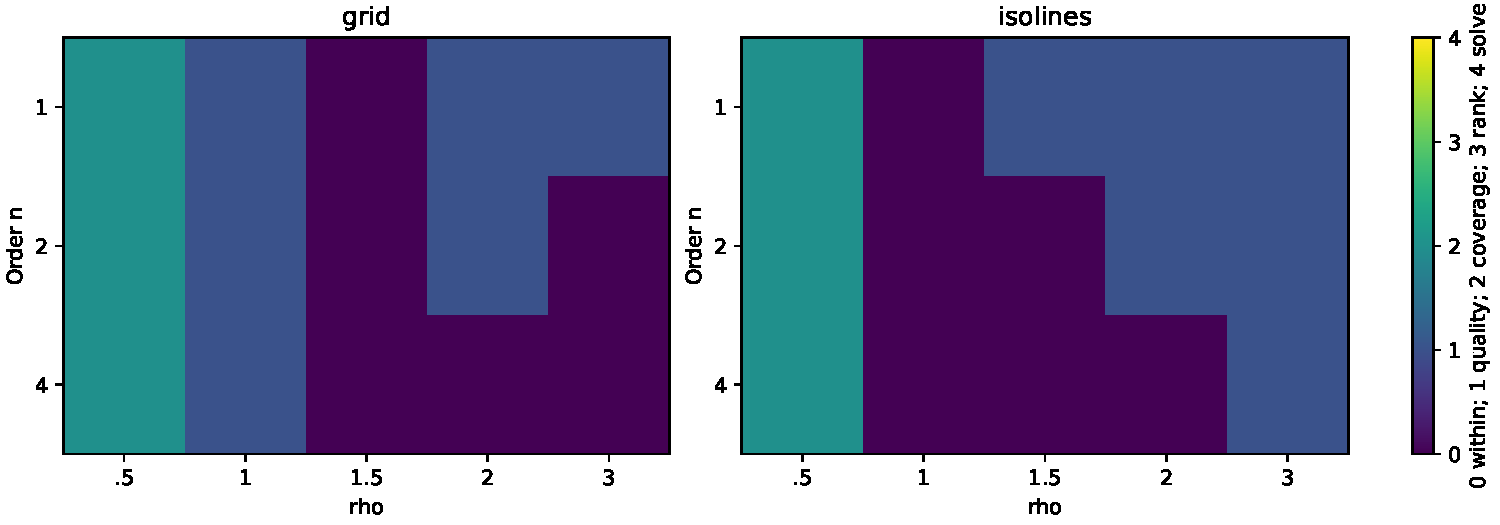
\includegraphics[width=\linewidth]{results/extended/failure_map.pdf}\end{center}

\section*{Час і пам'ять}
Кожен метод/розмір/розмірність запускається в окремому subprocess.
BLAS/OMP --- один потік, три побудови та три повтори кожної серії
256, 2048, 8192 запитів; показано медіани, raw samples збережено.
RSS вимірюється через Linux ru\_maxrss і включає нативні бібліотеки;
окремо записано імпортний baseline та приріст максимуму.
Нульовий приріст може означати, що імпортний максимум був більшим.
Витягування ізоповерхні виконується після обліку RSS запитів.
Число байтів поля --- лише числовий payload, а не вся пам'ять процесу.

\[
 T(B,Q)=T_{build}+B\,T_{query}(Q),\qquad B=1,10,100.
\]
Таблиці містять також projection time, solve time та повні витрати
для B; це вартість готового поля. Добір параметрів із пункту 4
оплачується додатково і не приховується в build time.
Окремо виміряно редагування: зсув SDF на $0.01,-0.01,0.02$.
Режим cached зберігає вузли й факторизацію; для isolines ці вузли
вже не обов'язково є найближчими до нової геометрії. Другий режим
повністю перебудовує поле й перевибирає вузли. Обидві якості та
три часові повтори записані. Для cubic також кешується not-a-knot
матриця, тож повторна факторизація не нав'язується лише конкуренту.
Вартість cached: $T_{prepare}+B(T_{update}+T_{query})$;
час повного rebuild наведено окремо. Записано числовий обсяг
L/U/перестановок, а фактична пам'ять редагування --- окремий peak RSS.
Реалізації Python/SciPy є дослідницькими; ці числа не визначають
граничну швидкодію всього класу алгоритмів.

Парето визначено окремо для 2D/3D за трьома цілями:
середня похибка офсетів, байти payload і час 8192 запитів.
Домінування потребує не гірших усіх цілей та строго кращої однієї.
Час підготовки й абсолютний RSS показано окремо, вони не підміняються
часом запиту й payload. Різні h входять до того самого простору вибору.
\begin{center}\small\resizebox{\linewidth}{!}{\begin{tabular}{lllllllllll}\toprule
D & Метод & $h$ & Похибка & Build, с & 8192, с & Update, с & Rebuild, с & Payload KiB & Peak MiB & Парето\\\midrule
2 & pg\_grid & 0.2 & 0.01937 & 0.001587 & 0.005271 & 4.491e-05 & 0.001185 & 2.82 & 186.4 & False\\
2 & pg\_isolines & 0.2 & 0.0205 & 0.003332 & 0.005123 & 4.571e-05 & 0.002894 & 2.82 & 186.4 & False\\
2 & wendland\_c2\_grid & 0.2 & 0.01681 & 0.003807 & 0.01471 & 6.669e-05 & 0.003312 & 2.82 & 186.4 & False\\
2 & wendland\_c2\_isolines & 0.2 & 0.01801 & 0.005017 & 0.00961 & 6.045e-05 & 0.004786 & 2.82 & 186.4 & False\\
2 & wendland\_c4\_grid & 0.2 & 0.0154 & 0.002302 & 0.007383 & 5.125e-05 & 0.001855 & 2.82 & 186.4 & True\\
2 & wendland\_c4\_isolines & 0.2 & 0.01969 & 0.004997 & 0.009525 & 6.027e-05 & 0.004438 & 2.82 & 186.4 & False\\
2 & linear & 0.2 & 0.04327 & 0.0002627 & 0.0002271 & 2.822e-05 & 6.058e-05 & 2.82 & 186.4 & True\\
2 & cubic & 0.2 & 0.01755 & 0.001418 & 0.001039 & 9.07e-05 & 0.000898 & 2.82 & 186.4 & True\\
2 & cubic\_redistance & 0.2 & 0.08276 & 0.001753 & 0.0002583 & 0.0004172 & 0.001223 & 10.7 & 186.4 & False\\
2 & pg\_grid & 0.3 & 0.03518 & 0.001379 & 0.004776 & 4.141e-05 & 0.0009017 & 2.258 & 186.4 & False\\
2 & pg\_isolines & 0.3 & 0.03001 & 0.003108 & 0.004769 & 4.112e-05 & 0.002431 & 2.258 & 186.4 & True\\
2 & wendland\_c2\_grid & 0.3 & 0.02994 & 0.002794 & 0.01427 & 5.422e-05 & 0.002355 & 2.258 & 186.4 & False\\
2 & wendland\_c2\_isolines & 0.3 & 0.01858 & 0.003981 & 0.008675 & 7.586e-05 & 0.004444 & 2.258 & 186.4 & True\\
2 & wendland\_c4\_grid & 0.3 & 0.02766 & 0.001862 & 0.006465 & 4.713e-05 & 0.001441 & 2.258 & 186.4 & True\\
2 & wendland\_c4\_isolines & 0.3 & 0.02471 & 0.003945 & 0.008673 & 4.84e-05 & 0.003387 & 2.258 & 186.4 & True\\
2 & linear & 0.3 & 0.06894 & 0.0002431 & 0.0002451 & 2.602e-05 & 7.23e-05 & 2.258 & 186.4 & True\\
2 & cubic & 0.3 & 0.03013 & 0.00123 & 0.001045 & 8.625e-05 & 0.0008515 & 2.258 & 186.4 & True\\
2 & cubic\_redistance & 0.3 & 0.1004 & 0.001753 & 0.0002464 & 0.0003346 & 0.001138 & 8.508 & 186.4 & False\\
3 & pg\_grid & 0.4 & 0.05987 & 0.06269 & 0.02162 & 0.001209 & 0.06236 & 26.37 & 186.4 & True\\
3 & pg\_isolines & 0.4 & 0.1145 & 0.08378 & 0.02185 & 0.001207 & 0.085 & 26.37 & 186.4 & False\\
3 & wendland\_c2\_grid & 0.4 & 0.06914 & 0.8563 & 0.09687 & 0.003891 & 0.831 & 26.37 & 186.4 & False\\
3 & wendland\_c2\_isolines & 0.4 & 0.09767 & 0.3842 & 0.04736 & 0.002437 & 0.5083 & 26.37 & 186.4 & False\\
3 & wendland\_c4\_grid & 0.4 & 0.07421 & 0.1828 & 0.03246 & 0.001828 & 0.1821 & 26.37 & 186.4 & False\\
3 & wendland\_c4\_isolines & 0.4 & 0.09455 & 0.3885 & 0.04781 & 0.002449 & 0.5072 & 26.37 & 186.4 & False\\
3 & linear & 0.4 & 0.1861 & 0.0003507 & 0.0005453 & 0.000111 & 0.0001881 & 26.37 & 186.4 & True\\
3 & cubic & 0.4 & 0.06634 & 0.09023 & 0.002423 & 0.002092 & 0.08844 & 26.37 & 186.4 & True\\
3 & cubic\_redistance & 0.4 & 0.1448 & 0.09841 & 0.0006182 & 0.01057 & 0.09844 & 190.5 & 186.4 & True\\
3 & pg\_grid & 0.5 & 0.1041 & 0.02648 & 0.01816 & 0.0005313 & 0.02634 & 17.16 & 186.4 & False\\
3 & pg\_isolines & 0.5 & 0.3135 & 0.04141 & 0.01807 & 0.0005349 & 0.04067 & 17.16 & 186.4 & False\\
3 & wendland\_c2\_grid & 0.5 & 0.09753 & 0.3131 & 0.1127 & 0.00201 & 0.3123 & 17.16 & 186.4 & False\\
3 & wendland\_c2\_isolines & 0.5 & 0.1244 & 0.2173 & 0.04222 & 0.001704 & 0.2084 & 17.16 & 186.4 & False\\
3 & wendland\_c4\_grid & 0.5 & 0.08395 & 0.1239 & 0.02926 & 0.001443 & 0.1196 & 17.16 & 186.4 & True\\
3 & wendland\_c4\_isolines & 0.5 & 0.1058 & 0.209 & 0.04301 & 0.001754 & 0.2088 & 17.16 & 186.4 & False\\
3 & linear & 0.5 & 0.1628 & 0.0003874 & 0.0005624 & 0.0001103 & 0.0001666 & 17.16 & 186.4 & True\\
3 & cubic & 0.5 & 0.0908 & 0.03124 & 0.002439 & 0.001244 & 0.02996 & 17.16 & 186.4 & True\\
3 & cubic\_redistance & 0.5 & 0.1723 & 0.03692 & 0.000577 & 0.006436 & 0.03513 & 122.1 & 186.4 & False\\
\bottomrule\end{tabular}}\end{center}
\begin{center}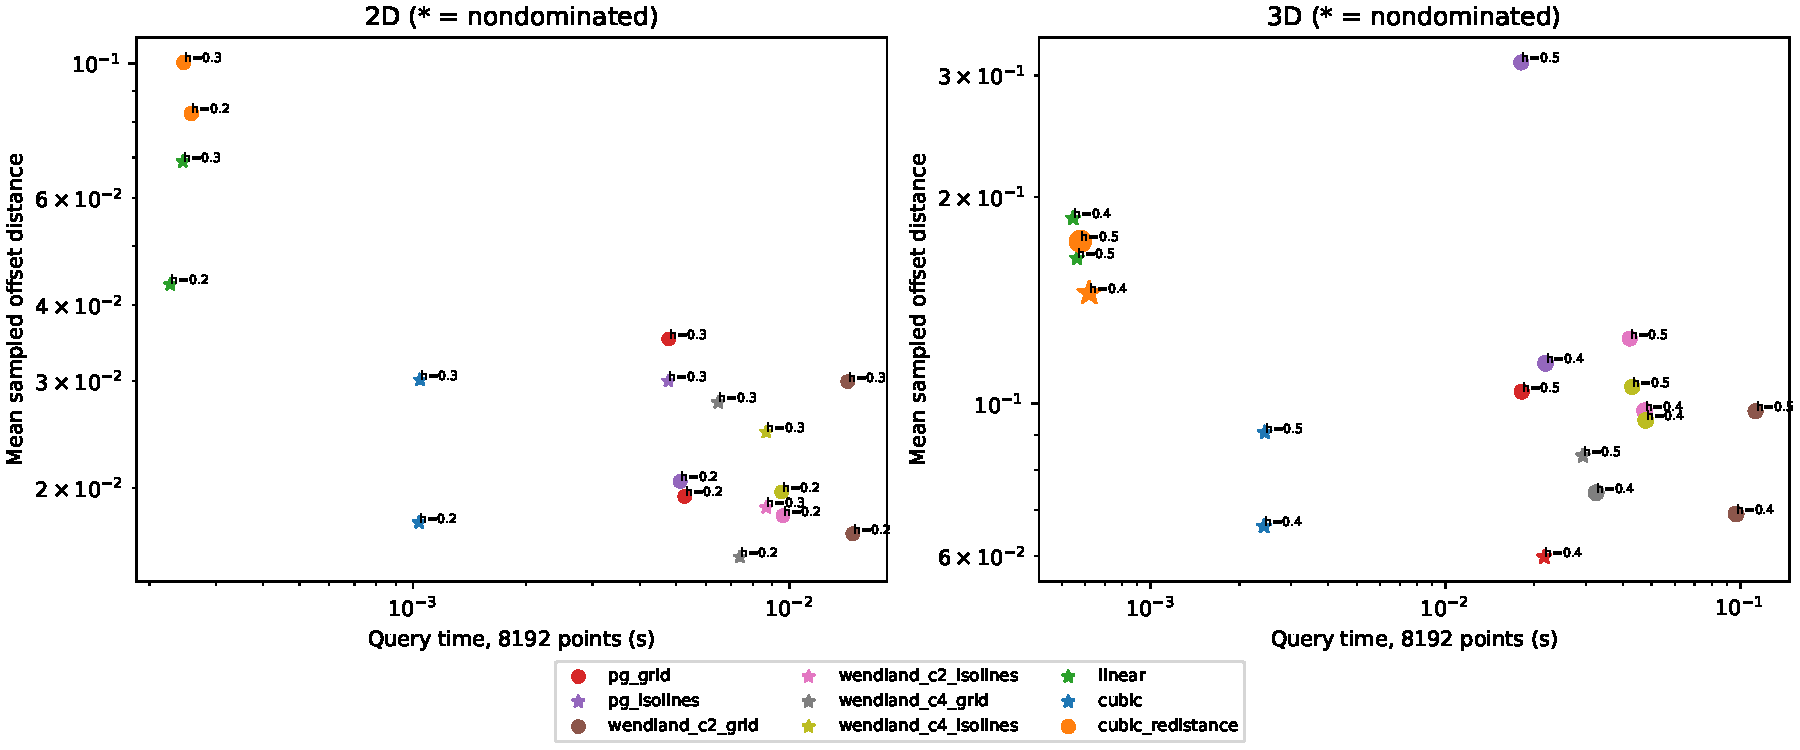
\includegraphics[width=\linewidth]{results/extended/pareto.pdf}\end{center}
\end{document}
